\documentclass[]{article}
\usepackage[a4paper]{geometry}
\usepackage{amssymb}
\usepackage{amsmath}
\usepackage{mathabx}
\usepackage{graphics}
%\usepackage{mathtools}
\usepackage{tikz}
\usepackage{array}
\usepackage{proof}
\usepackage{hyperref}
\definecolor{linkcolour}{rgb}{0,0.2,0.6}
\hypersetup{colorlinks,breaklinks,urlcolor=linkcolour,linkcolor=linkcolour}
\usepackage{subcaption}
\usetikzlibrary{calc, trees, fit, positioning}

\begin{document}
\author{Konstantinos Kogkalidis [6230067]}
\title{Recent Advancements in Neural Computation: \\
\large Differentiable Neural Computers and End-To-End Memory Networks}
\maketitle

\section{Introduction}
In the last decade, neural networks have considerably revolutionized computation and artificial intelligence. Neural networks have been setting new benchmarks in tasks from a broad range of fields, including computer vision, natural language processing and pattern recognition; many of these tasks previously unsolved, and some of these benchmarks surpassing human-level performance. Until recently, this astounding potential has for the most part been limited to tasks involving sensory processing and representation learning. Memory-centric tasks, i.e. tasks requiring data storage and retrieval, have however proven difficult for neural networks to model. This paper serves as a literature review of two recent approaches towards bypassing this limitation, namely Differentiable Neural Computers\cite{Graves2016} and End-to-End Memory Networks\cite{NIPS2015_5846}. The rest of this section will briefly introduce some important background concepts, before some notation is established in Section \ref{sec:Notation}. The models' details are examined in Sections \ref{DNC} and \ref{E2E}, respectively. Section \ref{Comp} provides a short discussion and a comparative analysis on the two approaches, and Section \ref{Conc} presents some concluding remarks.

A particularly interesting class of neural networks are \textit{Recurrent Neural Networks} (RNNs). Unlike fully-connected networks, which accept a fixed-size input vector and produce a fixed-size output vector over a finite number of computational steps, RNNs instead operate on sequences of vectors. This additional axis of dependencies is captured by a recurrency relation interlinking the network's hidden states through time. More concretely, the hidden representation is no longer conditioned on just the current input, but also on the immediately previous version of itself (Fig.\ref{fig:1}). This elegant addition accounts for a drastic improvement in the representational capacity of the network. Whereas a simple net acts as a trainable (but parametrically fixed) function, a RNN acts as a continuous program operating on sequences of inputs, and is in fact Turing complete\cite{Siegelmann545}. Under this viewpoint, the RNN's hidden representation can be perceived as the program's internal variables, updating as new inputs are received and affecting the computation as it progresses.

\begin{figure}
\begin{minipage}{0.5\textwidth}
	\centering
	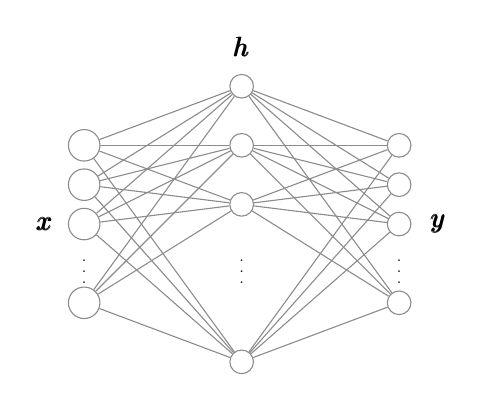
\begin{tikzpicture}[scale=0.5]
		\node (X) at (-1, -2) {$\pmb{x}$};
		\foreach \y /\alph/\name in {
			0/x1/{},
		  	-1/x2/{},
		  	-2/x3/{},
		  	-4/xM/{}
		 }{
		 	\node[circle, draw=gray!90, inner sep=0pt,minimum size=4mm,fill=white] (\alph) at (0,\y) {\tiny \textcolor{black}{\name}};
		 }
		 \node (H) at (4, 2.5) {$\pmb{h}$};
		 \node (x..) at (0,-3) {\tiny {\vdots}};
		 \foreach \y /\alph/\name in {
			1.5/h1/{},
		  	0/h2/{},
		  	-1.5/h3/{},
		  	-5.5/hN/{}
		 }{
		 	\node[circle, draw=gray!90, inner sep=0pt,minimum size=3mm,fill=white] (\alph) at (4,\y) {\tiny \textcolor{black}{\name}};
		 }
		 \node (h..) at (4,-3) {\tiny {\vdots}};
		 \node (Y) at (9, -2) {$\pmb{y}$};
		 \foreach \y /\alph/\name in {
			0/y1/{},
		  	-1/y2/{},
		  	-2/y3/{},
		  	-4/yP/{}
		 }{
		 	\node[circle, draw=gray!90,inner sep=0pt,minimum size=3mm,fill=white] (\alph) at (8,\y) {\tiny \textcolor{black}{\name}};
		 }
		 \node (y..) at (8,-3) {\tiny {\vdots}};
		 \foreach \x in {x1, x2, x3, xM}
		 {\foreach \h in {h1, h2, h3, hN}
		 {\draw (\x) edge[gray!90] (\h);}}
		 \foreach \x in {h1, h2, h3, hN}
		 {\foreach \y in {y1, y2, y3, yP}
		 {\draw (\x) edge[gray!90] (\y);}}
	\end{tikzpicture}
	\subcaption{Simple Neural Net}
	\end{minipage}
	\begin{minipage}{0.5\textwidth}
	\centering
	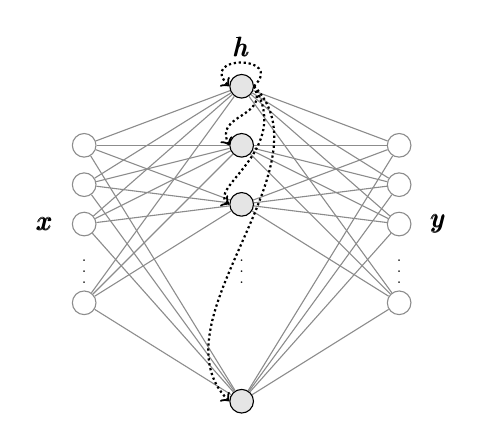
\begin{tikzpicture}[scale=.5]
		\node (X) at (-1, -2) {$\pmb{x}$};
		\foreach \y /\alph/\name in {
			0/x1/{},
		  	-1/x2/{},
		  	-2/x3/{},
		  	-4/xM/{}
		 }{
		% 	\node[] (\alph) at (0,\y) {\name};
		 	\node[circle, draw=gray!90, inner sep=0pt,minimum size=3mm,fill=white] (\alph) at (0,\y) {\tiny \textcolor{black}{\name}};
		 }
		 \node (x..) at (0,-3) {\tiny {\vdots}};
	  \node (H) at (4, 2.5) {$\pmb{h}$};
		 \foreach \y /\alph/\name in {
			1.5/h1/{},
		  	0/h2/{},
		  	-1.5/h3/{},
		  	-6.5/hN/{}
		 }{
		 	\node[circle, draw=black, inner sep=0pt,minimum size=3mm,fill=gray!20] (\alph) at (4,\y) {\tiny \textcolor{black}{\name}};
		 }
		 \node (h..) at (4,-3) {\tiny {\vdots}};
		 \node (Y) at (9, -2) {$\pmb{y}$};
		 \foreach \y /\alph/\name in {
			0/y1/{},
		  	-1/y2/{},
		  	-2/y3/{},
		  	-4/yP/{}
		 }{
		 	\node[circle, draw=gray!90, inner sep=0pt,minimum size=3mm,fill=white] (\alph) at (8,\y) {\tiny \textcolor{black}{\name}};
		 }
		 \node (y..) at (8,-3) {\tiny {\vdots}};
		 \foreach \x in {x1, x2, x3, xM}
		 {\foreach \h in {h1, h2, h3, hN}
		 {\draw (\x) edge[gray!90] (\h);}}
		 \foreach \x in {h1, h2, h3, hN}
		 {\foreach \y in {y1, y2, y3, yP}
		 {\draw (\x) edge[gray!90] (\y);}}
		 \draw (h1.east) [->, densely dotted, thick, black] .. controls +(0.8,0.8) and +(-0.8,0.8) .. (h1.west);
		 \draw (h1.east) [->, densely dotted, thick, black] .. controls +(0.4,-0.8) and +(-0.4,0.8) .. (h2.west);
		 \draw (h1.east) [->, densely dotted, thick, black] .. controls +(1,-1.6) and +(-0.6,0.4) .. (h3.west);
		 \draw (h1.east) [->, densely dotted, thick, black] .. controls +(2,-2) and +(-2,2) .. (hN.west);
\end{tikzpicture}
	\subcaption{Recurrent Neural Network}
	\end{minipage}
	\caption[]
	{\small \textit{Comparison between a feedforward neural network and a RNN. (a) The simple network applies two transformations $\pmb{x} \mapsto \pmb{h}$ and $\pmb{h} \mapsto \pmb{y}$, the composition of which can be seen as a function $\pmb{x} \mapsto \pmb{y}$. (b) The recurrent network allows through-time connections, depicted with the dotted lines, such that $\pmb{x}_t \times \pmb{h}_{t-1} \mapsto \pmb{h}_t$. The output then becomes a function of the full sequence of inputs received: $\underbrace{\pmb{x}_0 \times \pmb{x}_1 \times \dots \times \pmb{x}_t}_{\text{Sequence Length}} \mapsto \pmb{y}_t$.}\label{fig:1}}
\end{figure}

Although RNNs have been introduced more than three decades ago, their potential was only recognized recently, as the availability of computational power surged. Their ability to model sequential patterns and their interesting properties have garnered a lot of attention, yet they still suffer from two major drawbacks. The first relates to the statefulness achieved by their intermediate representation; even though it is distributed (hence more expressive than stochastic FSAs or Markov models)\cite[Lecture~10]{Hinton13}, the hidden vector's size is finite and fixed, therefore capable of only limited, lossy storage. The second is a more intrinsic one and is not only tied to RNNs but neural networks in general; there is no separation between memory and processing, as each neuron is simultaneously a minimal storage unit and a computational one. Although appealing from a biological perspective, this goes against the von Neumann model and the modern programming paradigm. 

A series of advancements has seeked to enhance RNNs with stronger memory management. Starting with the introduction of the \textit{Long Short-Term Memory}\cite{Hochreiter:1997:LSM:1246443.1246450,Gers99learningto}, which permits finite storage over very long computations, research in RNNs has bloomed towards many different directions. One particularly exciting recent advancement is the so-called \textit{attentional interface}\cite{NIPS2014_5542,Bahdanau} (Fig.\ref{fig:2}), which allows a network to selectively shift its focus on particular indices over a set of dimensions of an arbitrary tensor, thus enabling content-based adressing. The implications of this seemingly simple trick are tremendous; when employing fully differentiable attention (soft-attention), a network can learn how to pick out and combine relevant elements out of a (potentially very large) tensor, instead of lossily encoding it. This translates to arbitrary information retrieval; in other words, the same representations can now have different effects on the computation depending on the present context, similar to how a computer program would refer only to the variables dictated by its currently run instruction\cite{NIPS2014_5346}. Since its inception, attention has been a key-concept in many influential publications; the creative liberty it is offering, in terms of new potential operations, has also paved the way for architectures which decouple storage from computation. Such architectures, including but not limited to the two presented in this paper, utilize large external matrices and employ attention to perform read and write operations on them.

\begin{figure}
	\centering
	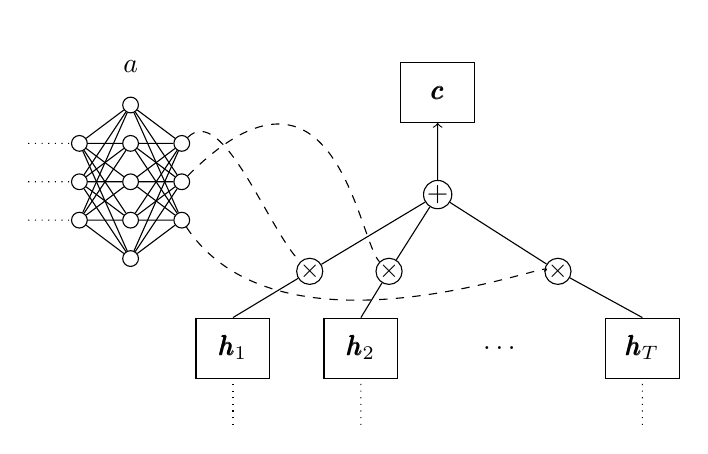
\begin{tikzpicture}
		[auto,
		scale=0.65,
		h/.style = {draw=black, rectangle, text centered, text depth=0.5em, text width = 2em, text height=1em,  align=center},
		c/.style = {draw=black, circle, minimum size=1mm, inner sep=0pt},
		c2/.style = {draw=black, circle, minimum size=2mm, inner sep=0pt}]
		
		
		\node (alpha) at (-2, 5.5) {$a$};
		\foreach \y/\alph in {
			4/Nx1,
			3.25/Nx2,
			2.5/Nx3}{
			\node[c2] (\alph) at (-3,\y) {};
		}
		\foreach \y/\alph in {
			4.75/Nh1,
			4/Nh2,
			3.25/Nh3,
			2.5/Nh4,
			1.75/Nh5}{
			\node[c2] (\alph) at (-2,\y) {};
		}
		\foreach \y/\alph in {
			4/Ny1,
			3.25/Ny2,
			2.5/Ny3}{
			\node[c2] (\alph) at (-1,\y) {};
		}		
			
		\foreach \source in {Nx1, Nx2, Nx3}{
		\foreach \target in {Nh1, Nh2, Nh3, Nh4, Nh5}{
			\draw (\source) edge (\target);}}
		\foreach \source in {Nh1, Nh2, Nh3, Nh4, Nh5}{
		\foreach \target in {Ny1, Ny2, Ny3}{
			\draw (\source) edge (\target);}}	
		
		
		\node (h..) at (5.25,0) {$\dots$};
		\foreach \x/\alph/\name in {
			0/h1/$\pmb{h}_1$,
			2.5/h2/$\pmb{h}_2$,
			8/hT/$\pmb{h}_T$
		}{
			\node[h] (\alph) at (\x,0) {\name};
		}
		\node[h] (c) at (4,5) {$\pmb{c}$};		
		
		\node[c] (+) at (4, 3) {$+$};
		
		\node[c] (x1) at (1.5,1.5) {\small $\times$};
		\node[c] (x2) at (3.05,1.5) {\small $\times$};
		\node[c] (xT) at (6.35,1.5) {\small $\times$};

		\draw (0,-1.5) edge[dotted] (h1);	
		\draw (2.5,-1.5) edge[dotted] (h2);	
		\draw (8,-1.5) edge[dotted] (hT);	
		\draw (h1.north) edge (x1);
		\draw (x1) edge (+);
		\draw (h2.north) edge (x2);
		\draw (x2) edge (+);
		\draw (hT.north) edge (xT);
		\draw (xT) edge (+);
		\draw (+) edge[->] (c);
		
		\draw (-4,4) edge[dotted] (Nx1);
		\draw (-4,3.25) edge[dotted] (Nx2);
		\draw (-4,2.5) edge[dotted] (Nx3);
		
		\draw (Ny1)  [dashed] .. controls +(0.8,0.8) and +(-0.8,0.8) ..  (x1);
		\draw (Ny2)  [dashed] .. controls +(3,3) and +(-0.6,0.6) ..  (x2);
		\draw (Ny3)  [dashed] .. controls +(2,-3) and +(0.6,0.4) ..  (xT.west);
	\end{tikzpicture}
	\caption[]
	{\small \textit{}\label{fig:2} General case of an attentional layer. Given some sequence $[\pmb{h}_1,\dots,\pmb{h}_T]$ (e.g. a full sequence of RNN hidden states), we may use an neural function $a$ to obtain a weighting vector $\pmb{a} \in \mathbb{R}^{T}$. Multiplying each sequence element by its corresponding weight and summing up the results, we end up with a context vector $\pmb{c}$. Note that when $a$ accepts an external vector (or vector sequence) as its argument, the result is a context-dynamic selection and linear combination of (parts of) the $[\pmb{h}_1,\dots]$ sequence.}
\end{figure}

\section{Notation and Preliminaries}
\label{sec:Notation}
Given the technical nature of the works presented, it is important to establish a notational common ground. The $(N-1)$-simplex, i.e. the set of all variations of $N$ non-negative scalars that sum up to 1, will be indicated by $\mathcal{S}^N$. A vector will be denoted by a boldface lower letter, e.g. $\pmb{v}$, whereas a matrix will be indicated by a boldface capital letter, e.g. $\pmb M$. Vector concatenation, i.e. merging together N vectors in the order they are given to a create a new, long vector is denoted by a bracketing of vectors separated by the semicolon, e.g. $[\pmb{x}; \pmb{y}; \pmb{z}]$ reads as the concatenation of $\pmb x$, $\pmb y$ and $\pmb z$. When using the comma rather than the semicolon, the notation instead presents a sequence of vectors, e.g. $[\pmb a _1, \dots ,\pmb a _N]$ denotes a sequence of vectors $\pmb a _1$ to $\pmb a _N$. A subscript on a vector or matrix is used to index a single temporal instance from a sequence of such vectors or matrices, e.g. $\pmb{a}_i$ refers to the instance at timestep $i$ of the time-varying vector sequence $[\pmb a _1 , \dots ]$. It should not be confused with intra-vector or matrix indexing, i.e. singling out particular elements out of a vector or matrix, which is denoted by $\pmb a [i]$ and reads as the i-th element of a vector $\pmb a$. Finally, a reminder that a matrix $\pmb M \in \mathbb{R}^{K\times L}$ can be seen as a linear map $M: \mathbb{R}^L \to \mathbb{R}^K$; linear application of $\pmb v \in \mathbb{R}^V $ on $\pmb M \in \mathbb{R}^{M \times V}$ (or matrix-vector multiplication) is thus simply denoted $\pmb {Mv}$.


\section{Differentiable Neural Computers}
\label{DNC}
\subsection{Description}
Inspired by the von Neumann architecture, DNCs model computation as the interfacing between two units; a RNN controller and an external memory matrix, functioning analogously to the CPU and the RAM, respectively. The memory matrix can be adressed using soft attention mechanisms, allowing selective reading and writing. As both the controller and the interfacing are differentiable, the full architecture is end-to-end differentiable, essentially allowing it to be trained purely with data and minimal human supervision. As the system is already equiped with the necessary tools to simulate traditional computation, i.e. adressing mechanisms, information storage and retrieval, logical flows and arithmetic processing, a DNC in training is learning the instructions of a program rather than the parameters of a function, and a trained DNC should be able to mimic the behavior of a traditionally hand-written program.

\subsection{Architecture}
\paragraph{Overview} 
A differentiable neural computer consists of two main components; a recurrent neural network, called the \textbf{controller network}, and an external \textbf{memory matrix} $M \in \mathbb{R}^{N\times W}$. The matrix contains $N$ memory adresses, each of size $W$, which can be read by the controller through $R$ \textit{read heads}, or written to by one \textit{write head}. At timestep t, the system as a whole receives input in the form of a vector, $\pmb{x}_t \in \mathbb{R}^X$, and produces output in the form of a vector, $\pmb{y}_t \in \mathbb{R}^Y$. The input may be samples from any dataset environment, e.g. some encoding of sensory signals. The output can either represent an approximation for a target vector $\pmb{z}_t \in \mathbb{R}^Y$ (in the supervised learning setting) or encode some action (in the reinforcement learning setting).

\begin{figure}
	\centering
	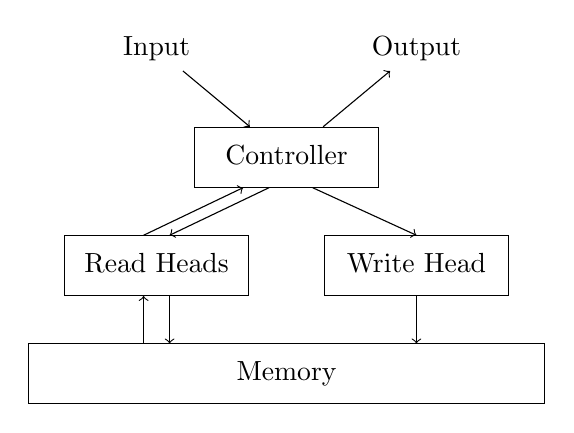
\begin{tikzpicture}
		[auto,
		scale=0.55,
		h/.style = {draw=black, rectangle, text centered, text depth=0.5em, text width = 6em, text height=1em,  align=center},
		c/.style = {draw=black, circle, minimum size=1mm, inner sep=0pt},
		c2/.style = {draw=black, circle, minimum size=2mm, inner sep=0pt}]
		
		\node[h, text width=18em] (memory) at (3,0) {Memory};		
		\foreach \x/\alph/\name in {
			0/read/{Read Heads},
			6/write/{Write Head}}
		{
			\node[h] (\alph) at (\x, 2.5) {\name};
		}
		\node[h] (controller) at (3,5) {Controller};\
		\node (input) at (0,7.5) {Input};
		\node (output) at (6,7.5) {Output};
		
		\draw (-0.3,0.7) edge[->] (-0.3,1.8);
		\draw (0.3,0.7) edge[<-] (0.3,1.8);
		\draw (6,0.7) edge[<-] (6,1.8);
		\draw (-0.3,3.2) edge[->] (2, 4.3);
		\draw (0.3,3.2) edge[<-] (2.6, 4.3);
		\draw (6,3.2) edge[<-] (3.6, 4.3);
		
		\draw (input) edge[->] (controller);
		\draw (controller) edge[->] (output);
		
	\end{tikzpicture}
	\caption[]
	{\small \textit{}\label{fig:3} High-level view of the DNC. The controller receives continuous input from some external source, which is processed and translated to memory reading/writing and computation instructions. During its operation, the DNC yields a continuous output stream back to the world.}
\end{figure}
\paragraph{Controller}
The aforementioned input is passed to the controller network, alongside the contents of each of the read heads as drawn from the memory at the previous time instance: $\pmb{r}_{t-1}^{i},\ i \in 1, \dots ,R$. The concatenation of the above yields a vector $\pmb{\chi}_t \in \mathbb{R}^{X + RW}: \pmb{\chi}_t = [\pmb{x}_t; \pmb{r}_{t-1}^1; \dots \pmb{r}_{t-1}^R ] $. A full sequence of such inputs, $[\pmb{\chi}_1,\dots ,\pmb{\chi}_T]$ is passed through a set of dynamic state equations $\mathcal{N}$, as implemented by the controller, that yield back two intermediate outputs, $\pmb{\upsilon }_T$ and $\pmb{\xi}_T$, such that $\mathcal{N}([\pmb{\chi}_1,\dots,\pmb{\chi}_T]) = (\pmb{\upsilon}_T,\ \pmb{\xi}_T)$. The exact implementation of $\mathcal{N}$ is not essential to the architecture as a whole; $\mathcal{N}$ may be any neural network. Deep long short-term memory networks are the state of the art in sequential modeling, and therefore make for a reasonable choice, since the controller needs to be expressive enough to handle potentially complex data streams.

Out of the vectors $(\pmb{\upsilon}_t,\ \pmb{\xi}_t)$ returned by the controller, the first corresponds to the intermediate user-level output. Before conveying this to the user, the system is allowed one last peak at the memory. This is necessitated by the fact that the read head contents at the final timestep of the computation cannot be used in $\mathcal{N}$, as this would introduce circular dependencies in the architecture's computational graph. The memory conditioning process is therefore done outside the controller, as captured by a simple trainable linear map \begin{equation}
\notag
\pmb{y}_t = \pmb{\upsilon}_t + \pmb{W}_R[\pmb{r}_{t}^1;\dots;\pmb{r}_{t}^R]
\label{eqn:Memory Conditioning}
\end{equation}
The result of the operation is the current instance of the user-level output stream, $\pmb{y}_t$, which represents what the DNC is yielding back to the world while computing. 

The second controller output, $\pmb{\xi}_t$, corresponds to the \textit{interface vector}, which defines the controller's interaction with the memory. The interface vector can be subvidided into multiple smaller components, each one of which is responsible for a specific subtask related to memory adressing. Different activation functions are applied to these components, forcing their distributions to lie within the domain dictated by their specific task. Post activation application, we have the following vectors and scalars:

\vspace{10pt}
\hspace{-40pt}
\begin{minipage}{0.6\textwidth}
\begin{itemize}
\item Read keys: \{$\pmb{k}_t^{r,i} \ \in \mathbb{R}^W, \ \forall i \in \{1,\dots,R\}$\}
\item Read strengths: \{$\beta_t^{r,i} \ \in [1, \infty) \ \forall i \in \{1,\dots,R\}$\}
\item Write key: $\pmb{k}_t^w \ \in \mathbb{R}^W$
\item Write strength: $\beta_t^w \ \in [1, \infty)$
\item Erase vector: $\pmb{e}_t \ \in [0,1]^W$
\end{itemize}
\end{minipage}
\hspace{-20pt}
\begin{minipage}{0.5\textwidth}
\begin{itemize}
\item Write vector: $\pmb{v}_t \ \in \mathbb{R}^W$
\item R free gates: \{$f_t^i \ \in [0,1] \ \forall i \in \{1,\dots,R\}$\}
\item Allocation gate: $g_t^a \ \in [0,1]$
\item Write gate: $g_t^w \ \in [0,1]$
\item Read modes: \{$\pmb{\pi}_t^i \ \in \mathcal{S}^3 \ \forall i \in \{1,\dots,R\}$\}
\end{itemize}
\end{minipage}
\vspace{10pt}

The remainder of this section is dedicated to examining the role of each of these components.

\paragraph{Content-based Addressing} 
DNCs perform content-based addressing via \textit{autoassociative memory}\cite[Chapter~12]{rojas}. Autoassociative memory is a strong mechanism of content-lookup, that allows a system to navigate rich data structures and selectively retrieve relevant memory objects when only shown parts thereof. The implementation involves a \textit{matching function} $\mathcal{D}: \mathbb{R}^W \times \mathbb{R}^W \to \mathbb{R}$, which is applied on a read/write key $\pmb{k}$, as given by the controller, and the contents of a memory address, $\pmb{M}[i,:]$, and returns a scalar indicating how similar these two are. Any metric of distance may be used as $\mathcal{D}$, but the most obvious choice is cosine similarity:
 \[
 \tag{Cosine Similarity} \label{eqn:Cosine}
\mathcal{D}(\pmb{x}, \pmb{y}) = cos(\pmb{x},\pmb{y}) = \frac{\pmb{x} \cdot \pmb{y}}{||\pmb{x}|| \cdot ||\pmb{y}||}
\]
The controller may assign varying relative importance on different keys; this is accomplished by raising the matches obtained by $\mathcal{D}$ to the strength vector associated with each key. These weighted matches are finally normalized by their sum, constraining the results within $\mathcal{S}^N$. The above are captured by a \textit{weighting function} $\mathcal{C}: \mathbb{R}^{N \times W} \times \mathbb{R}^W \times \mathbb{R} \to \mathbb{R}^N$, such that:
\[
\tag{Weighting Function}
\mathcal{C}(\pmb{M},\pmb{k}, \beta)[i] = 
\frac{ \mathcal{D}(\pmb{M}[i,:],\pmb{k})^{\beta} }
{\sum\nolimits_{j=1}^N \mathcal{D}(\pmb{M}[j,:],\pmb{k})^{\beta}}
\]

This is a fully differentiable form of attention, which allows the controller to construct minimal representations of objects that it's looking for in the memory. The key benefit of such a process is its ability to perform partial matching or pattern completion; for instance, the controller may simply construct the beginning of a sequence (e.g. the identifier of a variable), and, upon finding its match, it can then retrieve the full sequence (e.g. the  value of that variable) back from the memory.

The weighting function is used to obtain content-based weightings for both the read heads, denoted by $[\pmb{w}_t^{r,i},\dots,\pmb{w}_t^{r,R}]$, and the the write head, $\pmb{w}_t^w$. Given such weightings, a read head will contain a weighted average of the memory matrix:
\[
\tag{Memory Reading}
\pmb{r}_t^i = \pmb{M}_t^{\top} \pmb{w}_t^{r,i} 
\]
Writing to the memory is also dictated by a similar operation, which must now be defined via a recurrency relation to take into account past memory contents as well as the erase and write vectors emitted by the controller:
\[
\tag{Memory Writing}
\pmb{M}_t = \underbrace{\pmb{M}_{t-1} \circ (\pmb{1} - \pmb{w}_t^w \pmb{e}_t^\top)}_{\text{\scriptsize Partially erased past memory}} + \underbrace{\pmb{w}_t^w \pmb{v}_t^\top}_{\text{\scriptsize New memory}}
\]

\paragraph{Dynamic Allocation} Memory management is an integral part of any computer program. The DNC needs to be able to allocate and deallocate memory dynamically, according to the current execution's needs. This is achieved through a differentiable variation of the \textit{free-list scheme}. In its original form, the free-list scheme allows a system to keep track of unused memory blocks by connencting them with one another as a linked-list. Its adaptation for the purposes of the DNC is slightly more involved, as described next. Before writing to the memory, the controller emits a free gate, $f_t^i$, for each read head $i$, which controls to what extend a recently read memory address may be deallocated. From the latter, the \textit{retention vector} can be obtained as:
\[
\tag{Retention Vector}
\pmb{\psi}_t = \prod\limits_{i=1}^{R}{(\pmb{1}-f_t^i \pmb{w}_t^{r,i})}
\]

The retention vector is a measure of how much each memory address needs to be retained. Its functional complement, the \textit{usage-tracking vector} $\pmb{u}_t$, annotates each memory address with a scalar, responsible for signaling how strongly it is being used. It is recurrently defined as follows:
\[
\tag{Usage-tracking Vector}
\pmb{u}_t = \underbrace{(\pmb{u}_{t-1} + \pmb{w}_{t}^{w} - \pmb{u}_{t-1} \circ \pmb{w}_t^{w})}_{\text{ \scriptsize Previous usage OR New write}} \circ \ \pmb{\psi}_t
\]
Contrary to first impressions, the above equation is quite intuitive. The parenthesized term sums the previous usage tracking vector with the current write weighting minus their dot product, acting as a real-valued variation of the logical OR function. A single element of this term, $\pmb{u}_t[i]$ would denote the pre-retention usage tracking of memory address $i$; it is close to $1$ if it was either already in use, or just written to. Multiplied by its corresponding element of the retention vector, it can then be (partially) deallocated.
 
Finally, the free-list $\pmb{\phi}_t$ is defined as the sorted list of indices of the usage-tracking vector, i.e. $\pmb{\phi}_t[i]$ is the index of the i-th least used address in the memory. The \textit{allocation vector} $\pmb{a}_t$ is then  used to annotate the availability of each memory address:
\[
\tag{Allocation Vector}
\label{eqn:Allocation Vector}
\pmb{a}_t[\pmb{\phi}_t[j]] = (1 - \pmb{u}_t[\pmb{\phi}_t[j]])\prod\limits_{i=1}^{j-1}{\pmb{u}_t[\pmb{\phi}_t[i]]} \ \in [0,1]
\]

To showcase the functionality of this last equation, we will consider a simple example. Let $\pmb{u}_t = [0.4, 0.8, 0.1]$ be the usage-tracking vector of a 3-address memory at timestep $t$. Then the free-list would be $\pmb{\phi}_t = [3, 1, 2]$. Iterating over \ref{eqn:Allocation Vector} we then get:
\begin{align*}
\pmb{a}_t[\pmb{\phi}_t[1]] &= \pmb{a}_t[3] = (1-\pmb{u}_t[3]) \cdot 1 = (1-0.1) =0.9 \\
\pmb{a}_t[\pmb{\phi}_t[2]] &= \pmb{a}_t[1] = (1-\pmb{u}_t[1]) \cdot \pmb{u}_t[3] = (1 - 0.4) \cdot 0.1 = 0.06\\
\pmb{a}_t[\pmb{\phi}_t[3]] &= \pmb{a}_t[2] = (1-\pmb{u}_t[2]) \cdot \pmb{u}_t[3] \cdot \pmb{u}_t[1] = (1-0.8) \cdot 0.1 \cdot 0.4 = 0.008
\end{align*}
Therefore $\pmb{a}_t = [0.06, 0.08, 0.9]$. 

Having the allocation vector, the controller can now shift its attention towards unused memory addresses using the allocation gate $g_t^a$. The shifted weightings are then gated by the write gate $g_t^w$, which acts as a memory-locking mechanism :
\[
\tag{Allocation Shift}
\underbrace{\pmb{w}_t^w}_{\text{\scriptsize Updated weights}} = \underbrace{g_t^w}_{\text{Write-lock}} \quad [ \hspace{-10pt} \underbrace{g_t^a \pmb{a}_t}_{\text{\scriptsize Shifted weights}} + \underbrace{(1-g_t^w) \ \pmb{w}_t^w}_{\text{\scriptsize Writeable original weights}} \hspace{-15pt}]
\]

\paragraph{Temporal Linking} One last mechanism of memory addressing employed by DNCs is temporal linking. Temporal linking is necessary in order to perform sequential retrieval, when sequences are stored in disparate, non-contiguous blocks. The key-element of the process is a temporal transition matrix $\pmb{L} \in [0,1]^{N\times N}$, which keeps track of the temporal order by which memory addresses have been written to. More conretely, $\pmb{L}[i,j]$ is close to $1$ if $j$ was strongly written to after $i$, or close to $0$ otherwise. $\pmb{L}$ is again defined via a recurrency relation; a slightly simplified version of the one in the original paper is presented below, for the sake of brevity and clarity.
\[
\tag{Temporal Update}
\pmb{L}[i,j] = \underbrace{(1 - \pmb{w}_t^w[i] - \pmb{w}_t^w[j]) \pmb{L}_{t-1}[i,j]}_{\text{\scriptsize Part of last transition}} + \underbrace{\pmb{w}_{t-1}^w[i] \pmb{w}_{t}^w[j]}_{\text{\scriptsize New transition}}
\]
The above equation is also quite intuitive. The first term of the addition allows the transition value between $i$ and $j$ to propagate through time. The extend of propagation of the old transition, $\pmb{L}_{t-1}[i,j]$, is complentary to the amount of writing performed in these addresses; even if we had a transition in the past, it no longer holds if either $i$ or $j$ were just written to. On the other hand, if $i$ was written to in the previous timestep and $j$ was written to in the current timestep, then a new transition is instantiated. This is captured by the second term of the addition. 

\paragraph{Mode Interpolation} The temporal transition matrix can be used as one last means of attention; simply multiplying the matrix by a weighting vector allows the controller to shift its attention over the memory, now through time. $\pmb{L}_t \pmb{w}$ shifts the weightings $\pmb{w}$ forwards in time, whereas $\pmb{L}_t^\top \pmb{w}$ shifts them backwards. The degree to which the controller performs forward, backward, or no temporal iteration is dictated by the read modes $\pmb{\pi}_t^i$ emitted by the controller for each read head $i$:
\[
\tag{Temporal Shift}
\underbrace{\pmb{w}_t^{r,i}}_{\text{\scriptsize Updated weights}} \hspace{-10pt} = \quad
\underbrace{\pmb{\pi}_t^i[1] \pmb{L}_t\pmb{w}_t^{r,i}}_{\text{\scriptsize Forward shift}} + 
\underbrace{\pmb{\pi}_t^i[2] \pmb{w}_t^{r,i}}_{\text{\scriptsize No shift}} + 
\underbrace{\pmb{\pi}_t^i[3] \pmb{L}_t^\top \pmb{w}_t^{r,i}}_{\text{\scriptsize Backward shift}}
\]

\section{End-to-End Memory Networks}
\label{E2E}
\subsection{Description}
An end-to-end memory network is a neural architecture that also connects a RNN with a large memory array. The external nature of this array is disanalogous to traditional architectures, such as the LSTM, where the memory is encapsulated within the neural layers. Considering this difference, it can be perceived as true long-term memory. The memory can be read from (potentially multiple times) during computation, using a straightforward attentional layer; the architecture therefore benefits from context-sensitive addressing capabilities. The overall model is simple, yet efficient, and includes no discontinuities in its operations, thus being trainable with gradient-based methods.

\subsection{Architecture}
\paragraph{Overview}
An end-to-end memory network receives two inputs; a sequence of vectors $\{\pmb{x}_1,\dots,\pmb{x}_N\}$ and a query $\pmb{q}$. Both $\pmb{x}_i$ and $\pmb{q}$ are defined as symbols originating from a vocabulary $\mathcal{V}$. The network processes these inputs to return an answer $\pmb{a}$. This output is produced by first constructing continuous representations for both the input sequence and the query, and then iterating over these representations in many \textit{hops}, i.e. computational steps. The authors treat two different cases of this process; the first and simplest one employing a single layer, and the second, more general one, employing multiple layers. As this approach is favorable for understanding the architecture, we are also going to follow along the same route, modulo a few minor alterations and clarifications.

\paragraph{Single-Layer Case} First, note that a symbol $x$ from a strictly total-ordered vocabulary $\mathcal{V}$ can be uniquely represented as a vector $\pmb{x} \in \mathbb{R}^{V}$, where $V = ||\mathcal{V}||$ the size of the vocabulary. This is often referred to as \textit{one-hot encoding}. Given a character $x$ that coincides with the i-th element of $\mathcal{V}$, one-hot encoding is achieved by mapping $x$ to a vector $\pmb{x}$ whose elements are all $0$, except the $i$-th element which is $1$. This is the assumed form of input representation for the sequence $\{\pmb{x}_i\}$ and the query $\pmb{q}$. 

The above are transformed into two new, continuous spaces of dimensionality $d$; from each input $\pmb{x}_i$ we get a memory object $\pmb{m}_i$, whereas the query $\pmb{q}$ becomes an internal representation $\pmb{u}$. The transformations may be the result of any trainable operation, with the easiest choice being two \textit{embedding matrices} $\pmb{A}, \pmb{B} \in \mathbb{R}^{d\times V}$, such that:
\begin{align}
\pmb{m}_i &= \pmb{A}\pmb{x}_i \tag{Memory Transformation} \\
\pmb{u} &= \pmb{B}\pmb{q} \tag{Query Transformation}
\end{align}

As soon as we obtain the above, the matching vector $\pmb{p}$ between the query transformation and each memory object can be computed by passing the product of the two, $\pmb{u}^\top \pmb{m}_i$, through a Softmax activation:
\[
\tag{Memory Matching}
\pmb{p}_i = Softmax(\pmb{u}^\top \cdot \pmb{m}_i) = \frac{e^{\pmb{u}^\top\pmb{m}_i}}{\sum_j{e^{\pmb{u}^\top\pmb{m}_j}}}
\]
The inner product can be seen as a measure of similarity (reminiscent of \ref{eqn:Cosine}, minus the normalization), and the softmax activation is used to constrain $\pmb{p}$ within $\mathcal{S}^N$. 

A third transformation, via a third embedding matrix $\pmb{C} \in \mathbb{R}^{d\times V}$, is used to map inputs $\{\pmb{x}_i\}$ to their output representations $\{\pmb{c}_i\}$, from which the memory response can be derived as their match-weighted sum:
\begin{align}
\tag{Output Transformation}
\pmb{c}_i &= \pmb{C}\pmb{x}_i\\
\tag{Memory Response}
\pmb{o} &= \sum\limits_i{\pmb{p}_i\pmb{c}_i}
\end{align}

The ingenuity of this last equation is perhaps masked by its simplicity. It essentially accounts for a form of soft attention; the query dictates which parts of the output representation to focus on, depending on how it matched with the input representation. In other words, even though we always get the same output representation sequence $\{\pmb{c}_i\}$ from some input sequence $\{\pmb{x}_i\}$, the query $\pmb{q}$ plays an important role on how the network utilizes it.

Finally, the memory response is combined with the query representation through some binary operation (e.g. concatenation, element-wise addition or multiplication, etc.) and is passed through one last layer responsible for the final prediction. In the original paper, which assumes a classification setting, the authors propose a Softmax-activated linear map over the addition of the query and the response:
\[
\tag{Final Prediction}
\hat{\pmb{a}} = Softmax(\pmb{W} (\pmb{o}+\pmb{u}))
\]

Of course, this may be altered according to the requirements and restrictions imposed by the particular experimental environment. 

\paragraph{Multi-Layer Case}
In the more general case, the network may consist of multiple stacked layers; the presence of $K$ memory layers would then translate to $K$ hops. The authors propose a few different variations of connections between the different layers, which are summarized below. 

The first layer would operate as described in the previous paragraph. For each layer after the first, its input is defined as a linear combination of the previous layer's query and output transformations, i.e.
\[
\tag{Next Query}
\pmb{u}^{k+1} = \pmb{H}\pmb{u}^{k} + \pmb{o}^k 
\]
where $\pmb{H}$ may either be a trainable weight matrix (the same for all inter-layer links) or the identity matrix (in which case the query transformation is just added as is).

Each layer applies the memory and output transformations on $pmb{x}$ with each own embedding matrices $A^k, C^k$. The authors, however, explore a few options of weight-sharing in order to reduce the parameter space. One such option is to follow the RNN paradigm, letting all matrices with the same functionality be the same:
\[
\tag{RNN-Tying}
\forall \ (i,j): \pmb{A}^i = \pmb{A}^j, \pmb{C}^i = \pmb{C}^j
\]
This option is of particular interest, as then the network equations would be directly equivalent to those of RNNs, with one subtle but important difference. The intermediate representation $\pmb{p}$, which can be compared with the internal network recurrency, is not a static sample of the memory but rather a softly attended variant, which results in more expressive conditioning of the output on the memory. 

The other alternative proposed would be to tie these matrices in a way such that the memory representation of a layer is matched with the output representation of the previous one, in what the authors call adjacency tying. This can be achieved simply by letting:
\[
\tag{Adjacency Tying}
\pmb{A}^{k+1} = \pmb{C}^k
\]
What this accomplishes is constructing output representations that are continuous and comparable to the input representations of the immediately next layer, facilitating easier training.

\section{Discussion}
\label{Comp}
The previous sections have presented a summary of the design and functionality of two modern approaches towards enhancing recurrent networks with memory. This section will be devoted to some commentary on what the implications of these networks are, how they compare to one another and what their relevance is to computation as a whole.

\subsection{Comparisons}
Whereas both models are improvements over traditional recurrent networks, they approach the problem from two entirely different angles. 

Differentiable Neural Computers present a concrete, well-thought architecture that can simulate traditional computation via purely differentiable operations. This is one of the very first instantations of a model that falls within the domain of \textit{Probabilistic Programming}\cite{Meijer}, an emerging programming paradigm that proposes treating computer programs as stochastic distributions. Examined end-to-end, Differentiable Neural Computers propose a system capable of learning task-specific memory management and computation. Its practical use cases may be limited for the time being, but the contribution it makes as a whole is clear and rather groundbreaking; that of a single, unified machinery capable of learning programs with vastly different functionalities and input/output data structures; a great leap towards automated program inference. At the same time, the authors pose strong arguments for their design decisions and draw a few interesting parallels between biological intelligence and their system. 

Differentiable Neural Computers are the direct successor to Neural Turing Machines\cite{DBLP:journals/corr/GravesWD14}, a related architecture that has the same operative goals but slightly more limited functions. More specifically, Neural Turing Machines lack the ability to perform temporal linking and dynamic memory allocation. This limitation, in turn, disallows them from performing iterative memory retrieval of sequences stored in disparate blocks, and hinders their computational capacities when attempting to reiterate through a previously used memory matrix. Differentiable Neural Computers take specific measures against these problems, as described earlier, and thus excel at both memory allocation and arbitrary sequence retrieval.

End-to-End Memory Networks, on the other hand, make for a more grounded, applied approach. The proposal is far less convoluted and more compact in size, but its scope is also less ambitious. The overall focus seems to be on question answering tasks, even though the network is proposed as a general use architecture. Unlike Differentiable Neural Computers, no measures are taken towards program-centric capabilities; instead, a simple yet efficient mechanism of external memory attention is the paper's sole contribution. The exact implementation of this mechanism is clear and easy to follow, but feels somewhat arbitrary at times. For instance, no motivation is provided for the particular choices of transformations applied, both in terms of the concrete operations used, as well as their overall necessity. 

End-to-End Networks also draw inspiration from a predecessor paper, namely Memory Networks\cite{DBLP:journals/corr/WestonCB14}, which proposed a very similar architecture. Despite their similarity, End-to-End Networks make a very important contribution over the original paper. Whereas Memory Networks suffer from discontinuities and non-differentiable operations, requiring many levels of human supervision to train, End-to-End Networks resolve these issues by smart application of soft attention. Overall, the idea is easy to replicate and employ, serving as a portable and directly usable alternative to standard choices of sequence processing architectures such as the LSTM, at least for tasks requiring query matching and long-term data dependencies.

\subsection{Computational Relevance}
On another level, neither of the two papers address computation-theoretic problems. They are both very technical in nature, and their orientation is that of an engineering perspective. This does not, by any means, imply a weakness on their part. Neural Networks, and RNNs in particular, are already well-established as powerful machinery for function approximation\cite{Cybenko1989} and are known to be Turing complete\cite{SIEGELMANN1995132}. Improvements over their efficiency, training speed and applicability are nontheless extremely important scientific advancements, and as such both papers do progress the fields of both Artificial Intelligence and Computer Science. 

\section{Conclusion}
\label{Conc}
Machine learning has been called, often justifiably, an ad-hoc field, riddled with impulsive design decisions. Enhancing recurrent networks with memory capacities via attentive interfaces is a grounded, logical approach that seeks to shatter this perception. It is a far-reaching idea, deeply rooted in both modern computer science and neurological perspectives of biological intelligence. As such, I believe both of the papers presented are quite significant, as they pave the way for exciting new research and applications of neural computation.

In conclusion, fitting two lengthy technical papers into a brief overview is by no means an easy task. Several details had to be omitted, and some concessions had to be made on the amount of explanatory background provided. Nevertheless, I hope that this paper, as supplemented by the accompanying presentation, has managed to intrigue the interested reader and presented a motivating case towards further researching the topic. 

\bibliographystyle{ieeetr}
\bibliography{sources}

\end{document}
